\documentclass[landscape, two column, full page,leqno]{article}
\usepackage{mathrsfs}
\usepackage{amsmath,amssymb,amsthm}
%\usepackage[adobe-garamond]{mathdesign}
%\AtBeginDocument{%
%  \let\mathbb\relax
%  \DeclareMathAlphabet\PazoBB{U}{fplmbb}{m}{n}%
%  \newcommand{\mathbb}{\PazoBB}%
%  \let\mathcal\relax
%  \DeclareMathAlphabet{\OMScal}{OMS}{cmsy}{m}{n}
%  \newcommand{\mathcal}{\OMScal}%
%}
\usepackage{enumitem}
\usepackage{fontspec}
\usepackage{tikz}
\usetikzlibrary{arrows}
\usepackage{multicol}
\setmainfont[Numbers={Proportional,OldStyle}]{Adobe Garamond Pro}
\usepackage{fitch}
\usepackage{ND}
%SUBFIGURE PACKAGE
\usepackage{subfig}	
\usepackage[font=small]{caption}
\captionsetup[figure]{
labelfont=sc
}
\captionsetup[table]{
labelfont=sc
}
\captionsetup[subfloat]{%
font=footnotesize, labelfont=normalfont,
labelformat=parens,labelsep=space,
listofformat=subparens}
\captionsetup[subfigure]{font=footnotesize,
labelformat=parens,labelsep=space, labelfont=normalfont,
listofformat=subparens}
%GRAPHICX PACKAGE
\usepackage{graphicx}
\graphicspath{{C:/Users/jdg83/Dropbox/0000Desktop/Figures/}}
%NATBIB
\usepackage[comma]{natbib}
%HYPERREF PACKAGE
\usepackage{xcolor}
\PassOptionsToPackage{hyphens}{url}
\usepackage[backref=page,linktocpage=true,colorlinks]{hyperref}
\renewcommand{\backrefxxx}[3]{[\hyperlink{page.#1}{#1}]}
\hypersetup{
    colorlinks = true,
    citecolor = blue,
    urlcolor = blue,
    filecolor = blue,
    linkcolor = blue,
}
%PATCH TO ONLY HYPERLINK YEAR OF CITATION
\usepackage{etoolbox}
\makeatletter
% Patch case where name and year are separated by aysep
\patchcmd{\NAT@citex}
  {\@citea\NAT@hyper@{%
     \NAT@nmfmt{\NAT@nm}%
     \hyper@natlinkbreak{\NAT@aysep\NAT@spacechar}{\@citeb\@extra@b@citeb}%
     \NAT@date}}
  {\@citea\NAT@nmfmt{\NAT@nm}%
   \NAT@aysep\NAT@spacechar\NAT@hyper@{\NAT@date}}{}{}
% Patch case where name and year are separated by opening bracket
\patchcmd{\NAT@citex}
  {\@citea\NAT@hyper@{%
     \NAT@nmfmt{\NAT@nm}%
     \hyper@natlinkbreak{\NAT@spacechar\NAT@@open\if*#1*\else#1\NAT@spacechar\fi}%
       {\@citeb\@extra@b@citeb}%
     \NAT@date}}
  {\@citea\NAT@nmfmt{\NAT@nm}%
   \NAT@spacechar\NAT@@open\if*#1*\else#1\NAT@spacechar\fi\NAT@hyper@{\NAT@date}}
  {}{}
\makeatother
%
%Titlesec package
\usepackage{titlesec}
%Centering and readjusting size of headings
\titleformat{\section}[hang]
{\normalfont\sc\filcenter}{\thesection}{1em}{}
\titleformat{\subsection}[hang]
{\normalfont\sc\filcenter}{\thesubsection}{1em}{}
\titleformat{\subsubsection}[hang]
{\normalfont\sc\filcenter}{\thesubsubsection}{1em}{}
			% in the document preamble: 
				\let\endgraf\par % because LaTeX doesn't like \par 
			% in some command arguments 
				\let\subtitlefont\normalfont % or whatever 
				
%FOOTNOTE SPACING
\usepackage[hang,multiple,splitrule]{footmisc}
\setlength{\footnotemargin}{4mm}

\newcommand{\qd}{\begin{quote}\begin{description}  [align=left,style=nextline,leftmargin=*,labelsep=0pt,font=\normalfont]}
\newcommand{\zd}{\end{description}\end{quote}}
\newcommand{\qef}{\begin{enumerate}[leftmargin=0cm,labelsep=10pt]}
\newcommand{\qe}{\begin{enumerate}}
\newcommand{\qer}{\begin{enumerate}[align=left,style=nextline,leftmargin=17pt,labelsep=5pt,font=\normalfont , resume]}
\newcommand{\qei}{\begin{enumerate}[align=left,style=nextline,leftmargin=15pt, labelsep=10pt,font=\normalfont]}
\newcommand{\ze}{\end{enumerate}}
\newcommand{\p}{\item}
\newcommand{\e}{\emph}
\newcommand{\s}{\textsc}
\newcommand{\tbf}{\textbf}
\newcommand{\fn}{\footnote}
\newcommand{\argu}[2]{\begin{center}\begin{minipage}{#1} \begin{enumerate}
	#2
\end{enumerate}
\end{minipage}  
\end{center}}
\newcommand{\thus}{

\vspace{5pt}

\hrule

\vspace{-3pt}

}
%\newcommand{\fproof}[1]{\begin{center}\begin{fitch} #1 \end{fitch}\end{center}}
\newcommand{\qq}[1]{~\ulcorner #1  \urcorner~}
\newcommand{\V}[1]{\llbracket #1 \rrbracket}
\newcommand{\Va}[1]{\langle #1 \rangle}
\newcommand{\D}{\mathcal{D}}
\newcommand{\W}{\mathcal{W}}
\newcommand{\K}{\mathcal{K}}
\renewcommand{\u}{\mathfrak{u}}
\newcommand{\df}{\stackrel{\text{\tiny def}}{=}}
\newcommand{\fproof}[1]{\begin{center}\begin{fitch} #1 \end{fitch}\end{center}}
\usepackage{xcolor}
\usepackage{fancybox}

\definecolor{ShadowColor}{RGB}{30,150,190}

\makeatletter
\newcommand\Cshadowbox{\VerbBox\@Cshadowbox}
\def\@Cshadowbox#1{%
  \setbox\@fancybox\hbox{\fbox{#1}}%
  \leavevmode\vbox{%
    \offinterlineskip
    \dimen@=\shadowsize
    \advance\dimen@ .5\fboxrule
    \hbox{\copy\@fancybox\kern.5\fboxrule\lower\shadowsize\hbox{%
      \color{gray}\vrule \@height\ht\@fancybox \@depth\dp\@fancybox \@width\dimen@}}%
    \vskip\dimexpr-\dimen@+0.5\fboxrule\relax
    \moveright\shadowsize\vbox{%
      \color{gray}\hrule \@width\wd\@fancybox \@height\dimen@}}}
\makeatother

\newcommand{\csbox}[2]{\begin{center}
\Cshadowbox{
\begin{minipage}{#1}
	#2
\end{minipage}}
\end{center}
}


\title{Epistemic Externalism}
\date{November 13th, 2018}
\author{M\e{{\fontspec{Minion Pro} \&}}E Core}

\usepackage{layout}
\voffset = -40pt
\textheight = 450pt
\setlength{\columnsep}{20pt}
\begin{document}
%\layout
\twocolumn[{%
 \centering
\maketitle
}]

\section{Internalism and Externalism}
\qe
\p In general, an \e{internalist} says that some condition is within your epistemic reach---that, if the condition obtains, then you have some kind of access to the fact that the condition obtains.  As a general schema, we have:
	\begin{description}
	\item[$\mathcal{A}$-Internalism about $C$]  Necessarily, if condition $C$ obtains, then you have $\mathcal{A}$-access to the fact that $C$ obtains.
		\[
		\Box \left( C \to \mathcal{A} C\right)
		\] 
	\end{description}
	\qe
	\p For instance: if the condition is \e{that you believe that $\phi$} and the access is \e{belief}, then we get the internalist thesis that, necessarily, if you believe that $\phi$, then you believe that you believe that $\phi$,
		\[
		\Box( \mathcal{B} \phi \to \mathcal{BB} \phi )
		\]
	\p For another: if the condition is \e{that you are in pain}, $P$, and the access is \e{knowledge}, then we get the internalist thesis that, necessarily, if you are in pain, then you know that you are in pain,
		\[
		\Box( P \to \K P  )
		\]
	\p Or, if the condition is \e{that you know that $\phi$}, and the access is \e{knowledge}, then we get the internalist thesis that, necessarily, if you know that $\phi$, then you know that you know that $\phi$,
		\[
		\Box ( \K \phi \to \K \K \phi)
		\]
	\ze 
\p In general, an \e{externalist} says that some condition is \e{not} in your epistemic reach.  It is possible for the condition to obtain, even while you do \e{not} have access to the fact that the condition obtains.
	\begin{description}
	\item[$\mathcal{A}$-Externalism about $C$] Possibly, condition $C$ obtains and you do not have $\mathcal{A}$-access to the fact that $C$ obtains.
				\[
				\Diamond \left( C \wedge \neg \mathcal{A} C \right)
				\]
	\end{description}
	\qe
	\p For instance, if the condition is \e{that two words in your language are synonymous} and the access is \e{belief}, then we get the externalist thesis that it is possible for two words in your language to be synonymous even when you don't believe that they are.
	\p If the condition is \e{that the apple appears red to you}, $A$, and the access is \e{knowledge}, then we get the externalist thesis that it is possible for the apple to appear red to you without you knowing that the apple appears red to you,
			\[
			\Diamond (  A \wedge \neg \K A)
			\]
	\p If the condition is \e{that you know that $\phi$}, and the access is \e{knowledge}, then we get the externalist thesis that it is possible to know that $\phi$ without knowing that you know that $\phi$,
			\[
			\Diamond ( \K \phi \wedge \neg \K \K \phi )
			\]
	\ze 
	
\section{Anti-Luminosity}

\p Williamson argues for a strong version of externalism.  He accepts knowledge-externalism about $C$, \e{for all $C$}.  That is, for \e{every condition} $C$, it is possible that $C$ obtains even though you don't know that $C$.  Call this thesis `anti-luminosity'.
	\begin{description}
	\item[Anti-Luminosity]  For all conditions, $C$, it is possible that $C$ obtain without you knowing that $C$ obtains.
			\[
			\forall C \Diamond (C \wedge \neg \K C)
			\]
	\end{description}
	\qe
	\p If some condition $C$ is such that, necessarily, if $C$ obtains, then you know that $C$ obtains, then say that condition $C$ is \e{luminous}.  Anti-luminosity says that no condition is luminous.
	\ze 
\p This surprising conclusion follows from the apparently weak claim that knowledge is belief which is \e{safe from error}, together with the claim that we are incapable of discriminating very similar possibilities.
	\begin{description}
	\item[Safety] If you know that $\phi$, then, in similar possibilities, you don't falsely believe that $\phi$.
	\item[K $\subseteq$ J] If you know that $\phi$, then you have a justified belief that $\phi$.
	\item[Limited Discrimination] If you have a justified belief that $\phi$, then, in a similar possibility in which the basis of your belief is imperceptibly changed, you still believe that $\phi$.
	\end{description}
	\qe
	\p  \tbf{Safety} only provides a \e{necessary} condition for knowledge, and not a \e{necessary and sufficient} condition for knowledge.
	\p \tbf{Safety} \e{doesn't} say that, if you know that $\phi$, then, in nearby possibilities, $\phi$ is true.  That principle would be false, since I can know that mudrunner won even though he could have easily lost.  My belief is still safe from error, because, in the nearby possibilities in which he loses, I don't believe that he wins.
	\p  \tbf{Safety} does not clearly specify which possibilities are nearby.  However, Williamson will not need to do this in general in order to argue for \tbf{Anti-luminosity}.  He will need only to find, for each condition $C$, a sequences of cases, $w_0, w_1, \dots, w_N$ such that each $w_i$ is \e{clearly} similar enough to $w_{i+1}$.
	\p The same goes for \tbf{Limited Discrimination}.  He need only for, for each condition $C$, a sequence of cases, $w_0, w_1, \dots, w_N$ such that, in each $w_i$, if you believe that $C$ obtains in $w_{i}$, then you also believe that $C$ obtains in $w_{i+1}$.
	\ze 
\p Williamson argues that the claim that a condition is luminous can be made to conflict with the claim that knowledge is belief safe from error.  Take a candidate luminous condition: that you are cold, $C$.  Suppose that, in the early morning, and you are clearly cold, $C$.  The temperature slowly and imperceptibly rises, until, in midday, you are clearly not cold.  Then, we can have a sequence of possibilities, 
	\[
	w_0, w_1, w_2, \dots, w_{i-1}, w_{i}, w_{i+1}, \dots, w_{N-1}, w_N
	\]
such that $w_0$ is you in the morning, $w_N$ is you at midday, and the time separating each $w_i$ and $w_{i+1}$ is as small as you wish.
	\qe
	\p Note that these possibilities are \e{centered} worlds.
	\ze 
\p Let's use `$\langle \phi \rangle_i$' to stand for `in possibility $i$, $\phi$ is true', $w_i \in \langle \phi \rangle$.  By the stipulations of the case, we have:
	\qe
	\p[(\tbf{1})] In $w_0$, you are cold.    $\Va{C}_0$
	\p[(\tbf{2})] In $w_N$, you are not cold.   $\Va{\neg C}_N$.
	\ze  
\p  \tbf{Safety}, \tbf{Limited Discrimination}, and \tbf{K $\subseteq$ J} can be used to argue for a \e{margin-for-error} principle, (\tbf{M}).
	\begin{description}
	\item[(M)] For all $i$, if you know that you are cold in $w_i$, then you are cold in $w_{i+1}$.
			\[
			(\forall i) \left( \Va{\K C }_i \to \Va{ C }_{i+1} \right) 
			\]
	\end{description}
	\qe
	\p Suppose, for conditional proof, that you know that $C$ in possibility $w_i$.
	\p So, by (a) and \tbf{K $\subseteq$ J}, you have a justified belief that $C$ in $w_i$.
	\p And, by (a) and \tbf{Safety}, you don't falsely believe that $C$ in very similar possibilities.
	\p Additional assumption: $w_{i+1}$ is a very similar possibility. 
	\p By (c) and (d), you don't falsely believe that $C$ in $w_{i+1}$.
	\p By \tbf{Limited Discrimination}, (b), and (d),  you believe that $C$ in $w_{i+1}$.
	\p By (e) and (f), $C$ is true in $w_{i+1}$.
	\p Completing our conditional proof, we have that, if you know that $C$ in $w_i$, then you are cold in $w_{i+1}$, (\tbf{M}).
	\ze 
\p The punchline: (\tbf{M}) and (\tbf{L})---the \e{luminosity} of coldness---are inconsistent with (\tbf{1}) and (\tbf{2}).
	\begin{description}
	\item[(\tbf{L})] If you are cold, then you know that you are cold.
		\[
		(\forall i)  \left( \Va{C}_i \to \Va{\K C}_i \right)
		\]
	\end{description}
They are inconsistent because, by repeated appeal to (\tbf{M}) and (\tbf{L})---and \e{modus ponens}, (MP)---we can go from (\tbf{1}) to the negation of (\tbf{2}):
	\fproof{
\ftag{(1)}{	 \Va{\K C}_0				}& (\tbf{1})	\\
\ftag{(2)}{	 \Va{\K C}_0 \to \Va{C}_1	}& (\tbf{M})	\\
\ftag{(3)}{	 \Va{C}_1				}& 1, 2 (MP)	\\
\ftag{(4)}{	 \Va{C}_1 \to \Va{\K C}_1	}& (\tbf{L})		\\
\ftag{(5)}{	 \Va{\K C}_1			}	& 3, 4 (MP)	\\
\ftag{(6)}{	 \Va{\K C}_1 \to \Va{C}_2	}& (\tbf{M})		\\
\ftag{(7)}{	 \Va{C}_2				}& 5, 6 (MP)	\\
\ftag{(8)}{	 \Va{C}_2 \to \Va{\K C}_2	}& (\tbf{L})		\\
\ftag{(9)}{	 \Va{\K C}_2			}	& 7, 8 (MP)	\\
\ftag{(10)}{	 \Va{\K C}_2 \to \Va{C}_3	}& (\tbf{M})		\\
\ftag{(11)}{	 \Va{C}_3				}& 9, 10 (MP)	\\
\ftag{(12)}{	 \Va{C}_3 \to \Va{\K C}_3	}& (\tbf{L})		\\
\ftag{$\vdots$}{	   \vdots				} &		$\vdots$	\\
\ftag{(4\textsc{n}$-$3)}{ \Va{\K C}_{N-1}		}& 	4\textsc{n}-5, 4\textsc{n}-4 (MP)		\\
\ftag{(4\textsc{n}$-$2)}{	 \Va{\K C}_{N-1} \to \Va{C}_N	}& (\tbf{M})	\\
\ftag{(4\textsc{n}$-$1)}{ \Va{C}_N					}& 4\textsc{n}-3, 4\textsc{n}-2 (MP)	
	}
\p So, we must choose between (\tbf{1}), (\tbf{2}), (\tbf{M}), (\tbf{L}), and (MP).
	\qe
	\p (\tbf{1}) and (\tbf{2}) are justified by the setup of the case.  We should not deny that it is possible to go from being cold to not being cold. 
	\p (\tbf{M}) is justified by \tbf{Safety},  \tbf{K $\subseteq$ J}, and \tbf{Limited Discrimination}.  So denying (\tbf{M}) means denying one of these principles.
	\p (MP) is a valid inference schema---even according to trivalent logics like those of \L ukasiewicz and the supervaluationist.  
	\p So, Williamson concludes: we should reject (\tbf{L}).  It holds in \e{many} cases---but the principle is not true in general.  In particular: there are borderline cases of coldness such that, in those cases, we are cold without knowing that we are cold.  (Notice that this is an existentially quantified claim---as such, a supervaluationist can accept it as true while denying all instances of it.)
	\ze 
\p But wait---doesn't this argument look an awful lot like the \e{sorites} argument?  That argument is plainly unsound, so doesn't that give us some reason to think that \e{this} argument is unsound?
	\qe
	\p In a sense, that is precisely what Williamson is arguing: he is arguing that (\tbf{L}), like the tolerance principle---$(\forall n) (H(n) \to H(n-1))$---appears very plausible, but is actually false, because it has a false instance.  Just like with the tolerance principle, the false instance only appears in borderline cases where we can't know whether the antecedent is true or false.  This partly explains why the principle (\tbf{L}) can appear so plausible despite its falsehood.  
	\p However, we might think that Williamson has mis-diagnosed the falsehood.  Maybe it is not (\tbf{L}) but (\tbf{M}) which is in fact false.  
	\p In defense, Williamson suggests  that we  precisify all of the relevant terms.  When we this with the sorites, one of the premises---the relevant instance of the tolerance principle $(\forall n) (H(n) \to H(n-1))$---will be false.  However, when we do this in Williamson's case---for instance, in figure \ref{fig1}---the margin-for-error principle, (\tbf{M}),  will not be false.  Instead, the principle of luminosity, (\tbf{L}), will be.  (In figure \ref{fig1}, (\tbf{M}) is true at all worlds, but (\tbf{L}) is false at $w_5$.)
	\ze 


\pagebreak
\begin{figure}[t]
\twocolumn[{%
%\begin{figure}
\centering
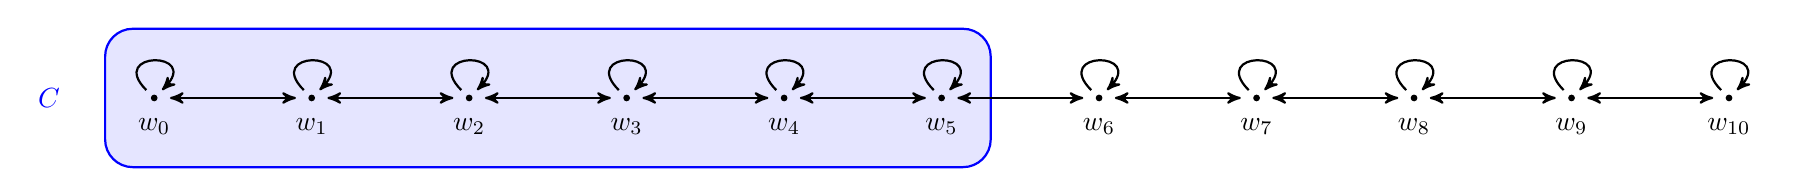
\begin{tikzpicture}[scale=2,>=stealth']
\tikzset{
%    p1/.style={%
%        draw=blue, thick,
%        rectangle,
%        rounded corners=10pt,
%        minimum height=100pt,
%        minimum width=30pt
%        },
    q1/.style={%
        draw=blue, thick,
        rectangle,
        rounded corners=10pt,
        minimum height=50pt,
        minimum width=320pt
        },
}
%%%PROPOSITIONS
%\node[p1, fill=blue, fill opacity=0.1] (c2) at (0,0.5) {};
\node[q1, fill=blue, fill opacity=0.1] (c1)  at (-2.5,0) {};
\filldraw[blue]  (-5.8, 0) node[anchor=west] { $C$ };
%\filldraw[blue]  (-0.55, 1) node[anchor=west] { $P$ };
%%%WORLDS
\filldraw [black] 
(-5,0) circle (0.5pt) node[anchor=north, below=4pt] { $w_0$ } 
(-4, 0) circle (0.5pt)   node[anchor=north, below=4pt] { $w_1$ } 
(-3,0) circle (0.5pt) node[anchor=north, below=4pt] { $w_2$ } 
(-2,0) circle (0.5pt)   node[anchor=north, below=4pt] { $w_3$ } 
(-1,0) circle (0.5pt) node[anchor=north, below=4pt] { $w_4$ } 
(0, 0) circle (0.5pt)   node[anchor=north, below=4pt] { $w_5$ } 
(1,0) circle (0.5pt) node[anchor=north, below=4pt] { $w_6$ } 
(2,0) circle (0.5pt)   node[anchor=north, below=4pt] { $w_7$ } 
(3,0) circle (0.5pt) node[anchor=north, below=4pt] { $w_8$ } 
(4, 0) circle (0.5pt)   node[anchor=north, below=4pt] { $w_9$ } 
(5,0) circle (0.5pt) node[anchor=north, below=4pt] { $w_{10}$ } 
;
%%%ACCESSIBILITY RELATIONS 
\draw[<->,thick] (-4.9, 0) -- (-4.1, 0);
\draw[<->,thick] (-3.9, 0) -- (-3.1, 0);
\draw[<->,thick] (-2.9, 0) -- (-2.1, 0);
\draw[<->,thick] (-1.9, 0) -- (-1.1, 0);
\draw[<->,thick] (-0.9, 0) -- (-0.1, 0);
\draw[<->,thick] (0.1, 0) -- (0.9, 0);
\draw[<->,thick] (1.1, 0) -- (1.9, 0);
\draw[<->,thick] (2.1, 0) -- (2.9, 0);
\draw[<->,thick] (3.1, 0) -- (3.9, 0);
\draw[<->,thick] (4.1, 0) -- (4.9, 0);
%
\draw[->, thick] (-5.05,0.05) .. controls (-5.3, 0.3) and (-4.7, 0.3) .. (-4.95, 0.05);
\draw[->, thick] (-4.05,0.05) .. controls (-4.3, 0.3) and (-3.7, 0.3) .. (-3.95, 0.05);
\draw[->, thick] (-3.05,0.05) .. controls (-3.3, 0.3) and (-2.7, 0.3) .. (-2.95, 0.05);
\draw[->, thick] (-2.05,0.05) .. controls (-2.3, 0.3) and (-1.7, 0.3) .. (-1.95, 0.05);
\draw[->, thick] (-1.05,0.05) .. controls (-1.3, 0.3) and (-0.7, 0.3) .. (-0.95, 0.05);
\draw[->, thick] (-0.05,0.05) .. controls (-0.3, 0.3) and (0.3, 0.3) .. (0.05, 0.05);
\draw[->, thick] (0.95,0.05) .. controls (0.7, 0.3) and (1.3, 0.3) .. (1.05, 0.05);
\draw[->, thick] (1.95,0.05) .. controls (1.7, 0.3) and (2.3, 0.3) .. (2.05, 0.05);
\draw[->, thick] (2.95,0.05) .. controls (2.7, 0.3) and (3.3, 0.3) .. (3.05, 0.05);
\draw[->, thick] (3.95,0.05) .. controls (3.7, 0.3) and (4.3, 0.3) .. (4.05, 0.05);
\draw[->, thick] (4.95,0.05) .. controls (4.7, 0.3) and (5.3, 0.3) .. (5.05, 0.05);
\end{tikzpicture}
\caption{{\small A precisified model in which you are cold, $C$, at worlds $w_1, w_2, w_3, w_4$, and $w_5$.  Because your perceptual capacities are limited, you cannot tell the difference between worlds $w_{i-1}, w_i,$ and $w_{i+1}$, for all $i \in \{ 1, 2, \dots, 9 \}$.  So, if you are at $w_i$, then for all you know, you are actually at $w_{i-1}$ or $w_{i+1}$ instead.   The margin-for-error principle (\tbf{M}) is true at all worlds in this model.  But the luminosity principle (\tbf{L}) is false at $w_5$, where you are cold, but, for all you know, you are not cold. \label{fig1}}}
\vspace{20pt}
%\end{figure}
}]
\end{figure}


\section*{The KK Principle}
\p Williamson thinks that this general argument  schema can be applied for any condition $C$.  If we let $C$ be the condition of knowing that $\phi$ is true, then we may argue against the claim that, if you know that $\phi$, then you know that you know that $\phi$.  Call this the `$KK$ principle':
	\[\tag{\tbf{KK}}
	\K \phi \to \K \K \phi
	\]
\p Here's a case which has received a fair bit of attention: suppose that you catch a brief glimpse of an ``irritatingly austere'' clock off in the distance (figure \ref{fig2a}).  
	\begin{figure}[h!]
	\centering
	\subfloat[\label{fig2a}]{	\includegraphics[scale=0.08]{williamsonclock20.eps}}
	\quad
	\subfloat[\label{fig2b}]{	\includegraphics[scale=0.08]{williamsonclock21.eps}}
	\quad
	\subfloat[\label{fig2c}]{	\includegraphics[scale=0.08]{williamsonclock22.eps}}
	\caption{}
	\end{figure}
The most you know about the position of the clock hand is that it is in some interval---call that interval $[a, b]$ (figure \ref{fig2b}).  Since you know that the hand lies in this interval, you know that it doesn't lie any \e{further} than $b$: 
	\qe
	\p[(\tbf{1})] $\K H \leq b$
	\ze 
And, since this is the \e{most} you know about the position of the clock hand, you don't know that the clock hand isn't at $b$:
	\qe
	\p[(\tbf{2})] $\neg \K H \neq b$
	\ze 
%(Here, `$H$' says `$x$ is the position of the clock hand'.)  
%
Additionally, you know enough about your discriminatory capacities in circumstances like this to know that, if the clock hand is at the position $b$, then you won't know that it lies in an interval which has $b$ as an endpoint (figure \ref{fig2c}).  (This is just a \e{margin-for-error} principle; we suppose here that it's not only true, but that you additionally \e{know} it to be true.)
	\qe
	\p[(\tbf{KM})] $\K \left[ H = b \to \neg \K H \leq b \right]$
	\ze 
The punchline: these assumptions---(\tbf{1}), (\tbf{2}), and (\tbf{KM})---are incompatible with (\tbf{KK}).    From (\tbf{1}), (\tbf{KM}), and (\tbf{KK}), we can derive the negation of (\tbf{2})
	\fproof{
	\ftag{(1)}{ \K \left[ H=b \to \neg \K H \leq b \right] }  & (\tbf{KM})	\\
	\ftag{(2)}{ \K \left[ \K H \leq b \to H \neq b \right]}	&1, contraposition	\\
	\ftag{(3)}{ \K \K H \leq b \to \K H \neq b }		&2, $K$-axiom		\\
	\ftag{(4)}{ \K H \neq b}						& (\tbf{1})		\\
	\ftag{(5)}{ \K H \neq b \to \K \K H \neq b}		& (\tbf{KK})	\\
	\ftag{(6)}{ \K \K H \neq b}					& 4, 5, modus ponens	\\
	\ftag{(7)}{ \K H \neq b }					& 3, 6, modus ponens	
	}
So, Williamson concludes, (\tbf{KK}) is false.
%But (7) contradicts (\tbf{2}). 

%\section{Clear Luminosity}
%\p Let the condition be \e{that you are clearly cold}.  Let the access be \e{knowledge}.  Then, we get the internalist thesis that, if you are clearly cold, then you know that you are clearly cold.
%	\[
%	\Box( \Delta C \to \K \Delta C)
%	\]
%Williamson will deny this principle for the same reason he denies 	
%	\[
%	\Box( \Delta C \to \K C)
%	\]
%	\[
%	\Box( \Delta \K \phi \to \K \K \phi)
%	\]
\ze 

\end{document}


